%%% BAT lecture 04 %%%
\documentclass{beamer}
\usepackage[utf8]{inputenc}
\usepackage{algorithm2e, amsmath, amssymb, amsfonts, graphicx}
% allow section.equation numbering
\numberwithin{equation}{section}
% use boadilla theme
\usetheme{Boadilla}
% remove navigation symbols
\usenavigationsymbolstemplate{}
% get numbered figure captions
\setbeamertemplate{caption}[numbered]
% changes itemize to circle + other things
\useoutertheme{split}
\useinnertheme{circles}

% command for the title string. change for each lecture
\newcommand{\lecturetitle}{Intro to Parametric Estimation}
% allow automatic alert-highlighted references and hyperlinks
\newcommand{\aref}[1]{\alert{\ref{#1}}}
\newcommand{\ahref}[2]{\href{#1}{\alert{#2}}}
% title page stuff. brackets content displayed in footer bar
\title[\lecturetitle]{\lecturetitle}
% metadata. content in brackets is displayed in footer bar
\author[Derek Huang (BAC Advanced Team)]{Derek Huang}
\institute{BAC Advanced Team}
\date{April 20, 2021}

% change "ball" bullet to numbered bullet and section title for section
\setbeamertemplate{section in toc}{\inserttocsectionnumber.~\inserttocsection}
% change ball to gray square (copied from stackoverflow; \par needed for break)
\setbeamertemplate{subsection in toc}{        
    \hspace{1.2em}{\color{gray}\rule[0.3ex]{3pt}{3pt}}~\inserttocsubsection\par}
% use default enumeration scheme
\setbeamertemplate{enumerate items}[default]
% required line that fixes the problem of \mathbf, \bf not working in beamer
% for later (post-2019) TeX Live installations. see the issue on GitHub:
% https://github.com/josephwright/beamer/issues/630
\DeclareFontShape{OT1}{cmss}{b}{n}{<->ssub * cmss/bx/n}{}

\begin{document}

% title slide
\begin{frame}
    \titlepage
    \centering
    % relative path may need to be updated depending on .tex file location
    
\includegraphics[scale = 0.1]{../bac_logo1.png}
\end{frame}

% table of contents slide
\begin{frame}{Overview}
    \tableofcontents
\end{frame}

% section
\section{Maximum likelihood}

\begin{frame}{Motivation}
    \begin{itemize}
        \item
        From last lecture, we saw how to fit the linear regression model.

        \item
        General method for fitting models?

        \item
        Are we making assumptions on the data distribution?
    \end{itemize}
    \begin{figure}[h!]
        \centering
        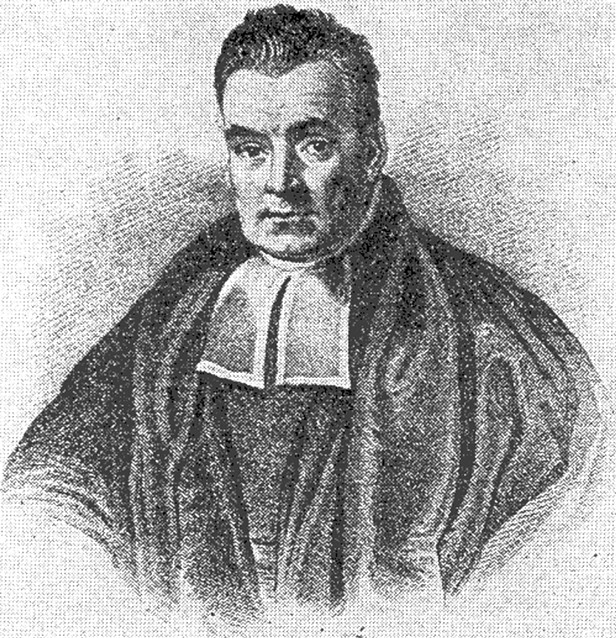
\includegraphics[scale = 0.18]{thomas_bayes.jpg}
        \caption{
            A portait of Thomas Bayes\footnote{
                The eponymous Bayes' theorem will prove to be useful
                throughout these slides.
            }.
        }
        \label{thomas_bayes}
    \end{figure}
\end{frame}

\subsection{MLE fundamentals}

\begin{frame}{MLE fundamentals}
    \begin{itemize}
        \item
        Let $ X : \Omega \rightarrow \mathbb{R}^d $ be the input variable,
        $ Y : \Omega \rightarrow \mathbb{R} $ be the response variable. Let
        $ \mathcal{D} \triangleq \{(\mathbf{x}_1, y_1), \ldots
        (\mathbf{x}_N, y_N)\} $ be the training data.

        \item
        Assume $ \mathbf{x}_1, \ldots \mathbf{x}_N $ are independently drawn
        from $ X $ and $ y_1 \ldots y_N $ are independently drawn from $ Y $.
        \textbf{Independence is a key assumption!}

        \item
        Assume a \textit{parametric model} for $ X, Y $ joint or $ Y \mid X $
        conditional distribution. That is, the distribution is parametrized
        by parameters $ \theta \in \Theta $, $ \Theta \subseteq \mathbb{R}^q $
        the \textit{parameter space}.

        \item
        Natural question: Given $ \theta $, how \textbf{likely} is it to
        sample $ \mathcal{D} $ from model?

        \item
        Natural maximization problem: Choose $ \hat{\theta} \in \Theta $, if
        $ \exists \hat{\theta} $, that maximizes the joint
        probability/density, or joint \textit{likelihood} of $ \mathcal{D} $.

        \item
        \textit{Remark. Notational abuse.} $ p $ often used to represent
        probabilities, densities, or mixtures of probabilities/densities.
        Be careful!
    \end{itemize}
\end{frame}

\begin{frame}{MLE fundamentals}
    \begin{itemize}
        \item
        \textit{Definition.} Given training data $ \mathcal{D} \triangleq
        (\mathbf{x}_1, y_1), \ldots (\mathbf{x}_N, y_N)\} $, each example
        drawn from the $ X, Y $ joint distribution, let
        \begin{equation*}
            p(\mathcal{D} \mid \theta) \triangleq p(\mathbf{x}_1, \ldots
                \mathbf{x}_N, y_1, \ldots y_N \mid \theta)
        \end{equation*}
        $ p(\mathcal{D} \mid \theta) $ is called the
        \textit{joint likelihood} of $ \mathcal{D} $.

        \item
        If $ D \triangleq [ \ X_1 \ \ldots \ X_N \ \ Y_1 \ \ldots
        \ Y_N \ ]^\top $ is a random variable with distribution
        parametrized by $ \theta $, $ p(\mathcal{D} \mid \theta) $ is the
        likelihood of observing $ \mathbf{x}_1, \ldots \mathbf{x}_N, y_1,
        \ldots y_N $. Note $ X_1, \ldots X_N $ i.i.d.,
        $ Y_1, \ldots Y_N $ i.i.d.

        \item
        Joint distributions are complicated. Can we simplify
        $ p(\mathcal{D} \mid \theta) $ somehow to make it easier to estimate?
    \end{itemize}
\end{frame}

\begin{frame}{MLE fundamentals}
    \begin{itemize}
        \item
        Yes, we use Bayes' rule on densities and the fact that our data
        examples $ (\mathbf{x}_1, y_1), \ldots (\mathbf{x}_N, y_N) $ are
        i.i.d.\footnote{
            To be precise, the examples are \textit{conditionally independent}
            given $ \theta $.
        }, so
        \begin{equation*}
            p(\mathcal{D} \mid \theta) =
            \prod_{k = 1}^N p(y_k, \mathbf{x}_k \mid \theta) =
            \prod_{k = 1}^N p(y_k \mid \mathbf{x}_k, \theta)
                p(\mathbf{x}_k \mid \theta)
        \end{equation*}

        \item
        Often only the $ Y \mid X $ conditional distribution is modeled so the
        distribution of $ X $ is independent of $ \theta $, i.e.
        $ p(\mathbf{x}_k \mid \theta) = p(\mathbf{x}_k) $. Then,
        \begin{equation} \label{cond_likelihood}
            p(\mathcal{D} \mid \theta) \propto
            \prod_{k = 1}^N p(y_k \mid \mathbf{x}_k, \theta)
        \end{equation}
        Here $ \propto $ means ``is proportional to''. We omit the
        $ p(\mathbf{x}_k) $ terms.
    \end{itemize}
\end{frame}

\subsection{Linear regression}

\begin{frame}{Linear regression}
    \begin{itemize}
        \item
        Let $ X : \Omega \rightarrow \mathbb{R}^d $,
        $ Y : \Omega \rightarrow \mathbb{R} $, be such that for
        $ \mathbf{w} \in \mathbb{R}^d $, $ b \in \mathbb{R} $,
        $ \sigma \in (0, \infty) $, $ \theta \triangleq (\mathbf{w}, b) $,
        $ Y \mid X, \theta \sim \mathcal{N}\left(
        \mathbf{w}^\top X + b, \sigma^2\right) $.

        \item
        Clearly the regression function is $ \mathbb{E}[Y \mid X, \theta] =
        \mathbf{w}^\top X + b $\footnote{
            Note $ \theta $ is treated like a random variable despite being
            fixed.
        }.

        \item
        The $ Y \mid X, \theta $ \textit{conditional density}
        $ p(y \mid \mathbf{x}, \theta) $ is simply
       \begin{equation} \label{linreg_density}
           p(y \mid \mathbf{x}, \theta) \triangleq
	           \frac{1}{\sqrt{2\pi}\sigma}
	           e^{-\frac{1}{2\sigma^2}\left(
	               y - \mathbf{w}^\top\mathbf{x} - b
               \right)^2}
       \end{equation}
       We can then rewrite (\aref{cond_likelihood}) more explicitly as
       \begin{equation} \label{linreg_like}
           p(\mathcal{D} \mid \theta) \propto
               \prod_{k = 1}^N\frac{1}{\sqrt{2\pi}\sigma}
               e^{-\frac{1}{2\sigma^2}\left(
                   y_k - \mathbf{w}^\top\mathbf{x}_k - b
               \right)^2}
       \end{equation}

        \item
        \textit{Remark.} As is typical, we will now treat
        $ p(\mathcal{D} \mid \theta) $ as a function of $ \theta $.
    \end{itemize}
\end{frame}

\begin{frame}{Linear regression}
    \begin{itemize}
        \item
        Note that $ \arg\max $ is invariant under monotone transformations. For
        example, if $ \hat{\theta} $ is the global maximum of
        $ p(\mathcal{D} \mid \theta) $,
        \begin{equation*}
            \hat{\theta} \triangleq \arg\max_\theta p(\mathcal{D} \mid \theta)
            = \arg\max_\theta \log p(\mathcal{D} \mid \theta)
        \end{equation*}

        \item
        Problems are equivalent, but $ \log p(\mathcal{D} \mid \theta) $ is a
        more convenient form (concave). Taking the log of (\aref{linreg_like})
        and collecting constants into $ C $,
        \begin{equation} \label{linreg_loglike}
            \log p(\mathcal{D} \mid \theta) = C - \sum_{k = 1}^N
                \frac{1}{2\sigma^2}\big(
                    y_k - \mathbf{w}^\top\mathbf{x}_k - b
                \big)^2
        \end{equation}

        \item
        $ \arg\max = -\arg\min $, $ \arg\max $ shift and positive scaling
        invariant $ \Rightarrow $
        \begin{equation} \label{linreg_like2cost}
            \hat{\mathbf{w}}, \hat{b} =
            \arg\max_{\mathbf{w}, b}\log p(\mathcal{D} \mid \mathbf{w}, b) =
            \arg\min_{\mathbf{w}, b}\sum_{k = 1}^N\big(
                y_k - \mathbf{w}^\top\mathbf{x}_k - b
            \big)^2
        \end{equation}
    \end{itemize}
\end{frame}

\subsection{Logistic regression}

\begin{frame}{Logistic regression}
    \begin{itemize}
        \item
        Let $ X : \Omega \rightarrow \mathbb{R}^d $, $ Y : \Omega \rightarrow
        \{-1, 1\} $, be such that for $ \mathbf{w} \in \mathbb{R} $,
        $ b \in \mathbb{R} $, $ \mathbb{P}\{Y = 1 \mid X, \theta\} =
        \sigma\big(\mathbf{w}^\top X + b\big) $, where $ \sigma : \mathbb{R}
        \rightarrow (0, 1) $ such that
        \begin{equation*}
            \sigma(z) = \frac{1}{1 + e^{-z}} = \frac{e^z}{1 + e^z} =
            1 - \frac{1}{1 + e^z}
        \end{equation*}

        \item
        $ \sigma $ is the \textit{sigmoid function}, use stems from the
        desire to model $ \mathbb{P}\{Y \mid X, \theta\} $ with affine
        functions \cite{esl}. Define $ \ell : (0, 1) \rightarrow \mathbb{R} $
        such that
        \begin{equation*}
            \ell(p) \triangleq \log\left(\frac{p}{1 - p}\right)
        \end{equation*}
        Let $ p_{+, \theta} \triangleq \mathbb{P}\{Y = 1 \mid X, \theta\} $.
        $ \frac{\sigma(z)}{1 - \sigma(z)} = e^z \Rightarrow
        \ell(p_{+, \theta}) = \mathbf{w}^\top X + b $.

        \item
        For any probability $ p \in (0, 1) $, $ \ell(p) $ are the
        \textit{log-odds}.
    \end{itemize}
\end{frame}

\begin{frame}{Logistic regression}
    \begin{itemize}
        \item
        Using our parametrization for $ \mathbb{P}\{Y = 1 \mid X, \theta\} $,
        we rewrite (\aref{cond_likelihood}) as
        \begin{equation*}
            p(\mathcal{D} \mid \theta) \propto
            \prod_{k = 1}^N\mathbb{P}\{Y = y_k \mid X = \mathbf{x}_k, \theta\}
        \end{equation*}
        Since $ \sigma(z) = \frac{1}{1 + e^{-z}} $, 
        $ 1 - \sigma(z) = \frac{1}{1 + e^z} $, then
        \begin{equation*}
            p(\mathcal{D} \mid \theta) \propto \prod_{k = 1}^N
            \sigma\big(y_k\big(\mathbf{w}^\top\mathbf{x}_k + b\big)\big)
        \end{equation*}

        \item
        Again\footnote{
            $ \arg\max $ invariant under monotone transformations,
            $ \arg\max = -\arg\min $.
        }, $ \hat{\theta} \triangleq \arg\max_\theta
        p(\mathcal{D} \mid \theta) = -\arg\min_\theta
        \log p(\mathcal{D} \mid \theta) $, so
        \begin{equation} \label{logreg_like2cost}
            \hat{\mathbf{w}}, \hat{b} = \arg\min_{\mathbf{w}, b}\sum_{k = 1}^N
            \log\left(1 + e^{-y_k(\mathbf{w}^\top\mathbf{x}_k + b)}\right)
        \end{equation}
    \end{itemize}

    % spacing for footnote
    \medskip
\end{frame}

\section{Maximum \textit{a posteriori}}

\subsection{MAP fundamentals}

\begin{frame}{MAP fundamentals}
    \begin{itemize}
        \item
        Maximum likelihood takes a \textit{frequentist} view towards parameter
        estimation, i.e. there is a true $ \theta^* $ that the data
        $ \mathcal{D} $ is sampled from.

        \item
        $ p(\mathcal{D} \mid \theta) \approx $ given $ \theta $, how likely is
        it to sample $ \mathcal{D} $?

        \item
        Maximum \textit{a posteriori} is a \textit{Bayesian} approach to
        parameter estimation, i.e. we treat $ \theta $ itself as a random
        variable.

        \item
        \textit{Definition.} $ p(\theta) $, the density/pmf of the parameter,
        is the \textit{prior}.

        \item
        MAP estimation considers the \textit{posterior}
        $ p(\theta \mid \mathcal{D}) $. Roughly, $ p(\theta \mid \mathcal{D}) 
        \approx $ given $ \mathcal{D} $, how likely is it to sample $ \theta $?

        \item
        $ p(\theta) $ reflects an initial guess for the distribution of the
        parameter while $ p(\theta \mid \mathcal{D}) $ reflects the
        distribution \textbf{conditional} on data $ \mathcal{D} $.
    \end{itemize}
\end{frame}

\begin{frame}{MAP fundamentals}
    \begin{itemize}
        \item
        How can we link the likelihood and prior? Bayes' rule gives us
        \begin{equation*}
            p(\theta \mid \mathcal{D}) =
            \frac{p(\mathcal{D} \mid \theta)p(\theta)}{p(\mathcal{D})} \propto
            p(\mathcal{D} \mid \theta)p(\theta)
        \end{equation*}

        \item
        We don't really care about $ p(\mathcal{D}) $, the marginal likelihood
        of the data, since $ \mathcal{D} $ is given and $ p(\mathcal{D}) $ is
        independent of $ \theta $.

        \item
        Clearly $ \log p(\theta \mid \mathcal{D}) = C +
        \log p(\mathcal{D} \mid \theta) + \log p(\theta) $, where $ C $
        collects any constant terms that don't depend on
        $ \mathcal{D}, \theta $.

        \item
        It's clear that MAP estimation amounts to tacking on the log prior to
        augment the objective function. Let's see a well-known example.
    \end{itemize}
\end{frame}

\subsection{Ridge regression}

\begin{frame}{Ridge regression}
    \begin{itemize}
        \item
        Recall (\aref{linreg_like}), the likelihood for the linear regression.
        Suppose the coefficients $ \mathbf{w} \sim \mathcal{N}(\mathbf{0},
        \nu^2\mathbf{I}) $, $ \nu > 0 $. The prior is then
        \begin{equation} \label{ridge_prior}
            p(\theta) \triangleq \frac{1}{(2\pi\nu^2)^{d / 2}}
            e^{-\frac{1}{2\nu^2}\mathbf{w}^\top\mathbf{w}}
        \end{equation}
        Since we didn't assume a distribution\footnote{
            Technically, no assumption amounts to assuming $ b $ is
            uniformly distributed over $ \mathbb{R} $.
        } on $ b $, $ b $ is omitted from
        (\aref{ridge_prior}).

        \item
        Taking the natural log and collecting constants with $ C $, we have
        \begin{equation*}
            \log p(\theta) = C - \frac{1}{2\nu^2}\mathbf{w}^\top\mathbf{w}
        \end{equation*}
        If we add $ \log p(\theta) $ to (\aref{linreg_loglike}), multiply
        by $ 2\sigma^2 $, and note $ \mathbf{w}^\top\mathbf{w} =
        \Vert\mathbf{w}\Vert_2^2 $,
        \begin{equation*}
            \log p(\theta \mid \mathcal{D}) = C - \sum_{k = 1}^N
            \big(y_k - \mathbf{w}^\top\mathbf{x}_k - b\big)^2 -
            \frac{\sigma^2}{\nu^2}\Vert\mathbf{w}\Vert_2^2
        \end{equation*}
    \end{itemize}
\end{frame}

\begin{frame}{Ridge regression}
    \begin{itemize}
        \item
        Let $ \lambda = \frac{\sigma^2}{\nu^2} $. $ \arg\max_\theta
        p(\theta \mid \mathcal{D}) =
        -\arg\min_\theta\log p(\theta \mid \mathcal{D}) $ and so
        \begin{equation}
            \hat{\mathbf{w}}_\lambda, \hat{b}_\lambda =
            \arg\min_{\mathbf{w}, b}\left\{\sum_{k = 1}^N
            \big(y_k - \mathbf{w}^\top\mathbf{x}_k - b\big)^2 +
            \lambda\Vert\mathbf{w}\Vert_2^2\right\}
        \end{equation}

        \item
        \textit{Remark.} Note that $ \lambda $ is inversely proportional to
        $ \nu $. Also, when $ \lambda $ increases, i.e. $ \nu $ is decreased,
        there is a greater penalty applied to nonzero coefficients in the
        objective.

        \item
        Increasing $ \lambda \Rightarrow $ assumption that $ \mathbf{w} $ is
        more tightly concentrated around $ \mathbf{0} \Rightarrow $ greater
        shrinkage of OLS coefficients.
    \end{itemize}
\end{frame}

\subsection{Regularization}

\begin{frame}{Regularization}
    \begin{itemize}
        \item
        In the context of MAP estimation, regularization amounts to assuming a
        prior distribution for $ \theta $. Therefore, there are simple
        probabilistic interpretations for popular regularizers.

        \item
        $ \ell^2 $-norm regularization of the form
        $ \lambda\Vert\mathbf{w}\Vert_2^2 $ for coefficients $ \mathbf{w} \in
        \mathbb{R}^p \Rightarrow \mathbf{w} \sim
        \mathcal{N}(\mathbf{0}, \alpha\mathbf{I}) $, where
        $ \alpha \propto \lambda^{-1} $. More generally, for
        $ \mathbf{Q} \triangleq \operatorname{diag}(\alpha_1, \ldots \alpha_p)
        \succ \mathbf{0} $, $ \mathbf{v} \in \mathbb{R}^p $,
        $ \alpha \propto \lambda^{-1} $,
        \begin{equation*}
            \lambda\Vert\mathbf{Q(w - \mathbf{v})}\Vert_2^2 \Rightarrow
            \mathbf{w} \sim \mathcal{N}\big(
                \mathbf{v}, \alpha\mathbf{Q}^{-1}\mathbf{Q}^{-1}
            \big)
        \end{equation*}

        \item
        $ \ell^1 $-norm regularizer $ \lambda\Vert\mathbf{w}\Vert_1 \Rightarrow
        w_1, \ldots w_p \sim \operatorname{Laplace}(0, \gamma) $, where
        $ \gamma \propto \lambda^{-1} $ and $ w_1, \ldots w_p $ mutually
        independent. The prior is
        \begin{equation*}
            p(\mathbf{w}) = \prod_{j = 1}^p\frac{1}{2\gamma}
            e^{-\frac{1}{\gamma}|w_j|}
        \end{equation*}
    \end{itemize}
\end{frame}

%\section{Appendix}
%
%\subsection{Multiclass logistic regression}
%
%\begin{frame}{Multiclass logistic regression}
%    \begin{itemize}
%        \item
%        \textit{Multiclass logistic regression.} $ \mathbf{X} \in
%        \mathbb{R}^{N \times d} $ is the input matrix, $ \mathcal{C}
%        \triangleq \{\mathcal{C}_1, \ldots \mathcal{C}_K\} $ a partition of
%        $ \mathbb{R}^n $. $ \mathbf{Y} \in \mathbb{R}^{N \times K} $ is the
%        an indicator matrix where $ \mathbf{x}_i \in \mathcal{C}_j \Rightarrow
%        y_{ij} = 1 $. $ \mathbf{W} \in \mathbb{R}^{d \times K} $ where column
%        $ \mathbf{w}_j $ gives $ j $th class weights and
%        $ \mathbf{b} \in \mathbb{R}^K $ be the vector where each
%        $ b_j $ is the $ j $th class intercept.
%
%        \item
%        Define $ \sigma_j : \mathbb{R}^{d \times K} \times \mathbb{R}^d \times
%        \mathbb{R}^K \rightarrow (0, 1) $ s.t. for $ j \in \{1, \ldots
%        |\mathcal{C}|\} $, $ \mathbf{x} \in \mathbb{R}^d $,
%		\begin{equation*}
%		    \sigma_j(\mathbf{W}, \mathbf{x}, \mathbf{b}) = \frac{
%		        e^{\mathbf{w}_j^\top\mathbf{x} + b_j}
%		    }{\sum_{k = 1}^K e^{\mathbf{w}_k^\top\mathbf{x} + b_k}}
%		\end{equation*}
%		For $ \lambda \in [0, \infty) $, the multi-class loss functional
%        $ J_\mathcal{D} : \mathbb{R}^{d \times |\mathcal{C}|} \rightarrow
%        [0, \infty) $, with data $ \mathcal{D} \triangleq
%        (\mathbf{X}, \mathbf{Y}) $, is then such that \cite{bishop_ml}
%		\begin{equation} \label{logreg_multiclass}
%		    J_\mathcal{D}(\mathbf{W}) = -\sum_{i = 1}^N\sum_{j = 1}^K
%		        y_{ij}\log\sigma_j(\mathbf{W}, \mathbf{x}, \mathbf{b})
%		        + \lambda\Vert\mathbf{W}\Vert_{\operatorname{F}}^2
%		\end{equation}
%    \end{itemize}
%\end{frame}

% BibTeX slide for references. should use either acm or ieeetr style
\begin{frame}{References}
    \bibliographystyle{acm}
    % relative path may need to be updated depending on .tex file location
    \bibliography{../master_bib}
\end{frame}

\end{document}